\documentclass{beamer}
\usepackage{listings}
\usepackage{parskip}
\lstset{
%language=C,
frame=single, 
breaklines=true,
columns=fullflexible
}

\usepackage{subcaption}
\usepackage{url}
\usepackage{tikz}
\usepackage{tkz-euclide} % loads  TikZ and tkz-base
%\usetkzobj{all}
\usetikzlibrary{calc,math}
\usepackage{float}
\newcommand\norm[1]{\left\lVert#1\right\rVert}
\providecommand{\pr}[1]{\ensuremath{\Pr\left(#1\right)}}
\renewcommand{\vec}[1]{\mathbf{#1}}
\usepackage[export]{adjustbox}
\usepackage[utf8]{inputenc}
\usepackage{amsmath}
\usetheme{Boadilla}

\title[MA4240 - Applied Statistics]{Mobile Phone Usage and Digital Wellbeing}
\subtitle{MA4240 - Applied Statistics}

\author[Group Project No: 3]{Himanshu~Jindal \and 
  Naman~Chhibbar \and
  Kaustubh Dandegaonkar\and
  Deepinder~Singh \and
  Shubham~Vishwakarma \and
  Roshan~Kumar \and
  Devashish~Chaudhari \and
  Karthik Dhanavath
  }
\date{\ May 3, 2023}
\begin{document}

\begin{frame}
\titlepage
\end{frame}

\begin{frame}{Outline}
    \begin{enumerate}
    \item{Introduction}
    \item{Data Visualization}
    \item{Data Analysis and Conclusions}
    \item{Confidence Intervals}
    \item{Hypothesis Testing}
    \item{Takeaways from the analysis}
\end{enumerate}
\end{frame}


\begin{frame}
\frametitle{Introduction}
\begin{block}{}
The impact of smartphone screen time on students’ physical health, mental health, and academic performance is investigated in our study. We performed a survey
to gather information about students’ smartphone screen time habits and perceived effects.
The collected data is statistically analyzed to determine the association between smartphone
screen time and its impacts. Our findings will provide vital insights into the possible hazards of excessive smartphone screen time and the significance of balancing a good lifestyle with other pursuits.
\end{block}
\end{frame}

\begin{frame}
\begin{block}{Points of interest}
\begin{enumerate}
\item What is your average screen time in a day?
\item How many times do you check your phone in a day?
\item How many notifications do you receive in a day?
\item What percentage of your screen time is productive?
\item What is the average time you study daily (outside college hours)?
\item How much do you usually study in one sitting? (Hours)
\item Which hostel are you staying in?
\item Which degree are you pursuing?	
\item Which year are you currently in?	
\item Gender of the student.	
\item Do you wear spectacles?	
\item Do you use the phone in class?	
\item Do you attend classes?	
\item How do you rate your focus?	
\item How do you rate your happiness or mental well-being?
\end{enumerate}
\end{block}
\end{frame}

\begin{frame}
\begin{block}{Pre-Processing of Data}
The following steps were taken to pre-process the data:
\begin{enumerate}
\item We started by removing white spaces in columns containing string values.
\item Missing values (NaNs) were replaced with the median value in the case of numerical, and with modal values in the case of categorical variables.
\item Categorical data like "between n and n+1" is replaced with n+(1/2) to make it numerical.
\item String data like "hostel" is replaced with the corresponding numerical index to make calculations easier.
\end{enumerate}
\end{block}
    
\end{frame}

\begin{frame}
\frametitle{Data Visualization}
\begin{block}{Analyzing the Uni-variate Numerical dataset}
\begin{center}
\captionof{table}{What is your average screen time in a day?}
\begin{tabular}{|c|c|}
\hline 
Count & 106(non-null) \\ 
\hline 
Mean & 5.96 \\ 
\hline 
Median & 5 \\ 
\hline 
Mode & 5 \\ 
\hline 
std & 3.52 \\ 
\hline 
25\% & 4 \\ 
\hline 
50\% & 5 \\ 
\hline 
75\% & 6.75 \\ 
\hline 
95\% Confidence Interval & (5.28,6.63) \\ 
\hline
99\% Confidence Interval & (5.06,6.85) \\ 
\hline
\end{tabular} 
\end{center}
\end{block}
\end{frame}

\begin{frame}
\begin{block}{Focus v/s screen-time}
\begin{figure}[hbtp]
\caption{Focus[1 to 5] v/s screen-time}
\centering
\includegraphics[scale=0.5]{Focus_vs_Screen_time.png}
\end{figure}
\end{block}
\end{frame}

\begin{frame}
\begin{block}{Number of times phone checked in a day}
\begin{figure}[hbtp]
\caption{Distribution of number of times phone checked by students}
\centering
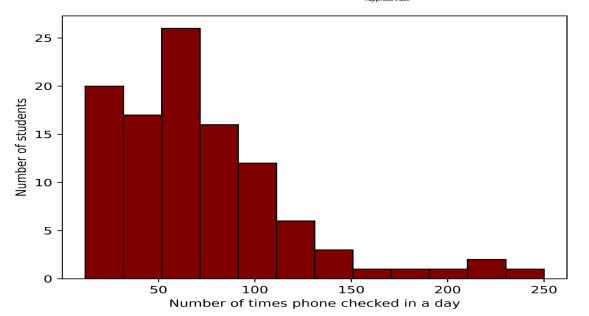
\includegraphics[width = 0.9\textwidth, height=6cm]{phone_check.png}
\end{figure}
\end{block}
\end{frame}

\begin{frame}
\begin{block}{Data Visualization with Segmented Bar plots}
\begin{figure}[hbtp]
\caption{Categorical variables in a segmented bar plot}
\centering
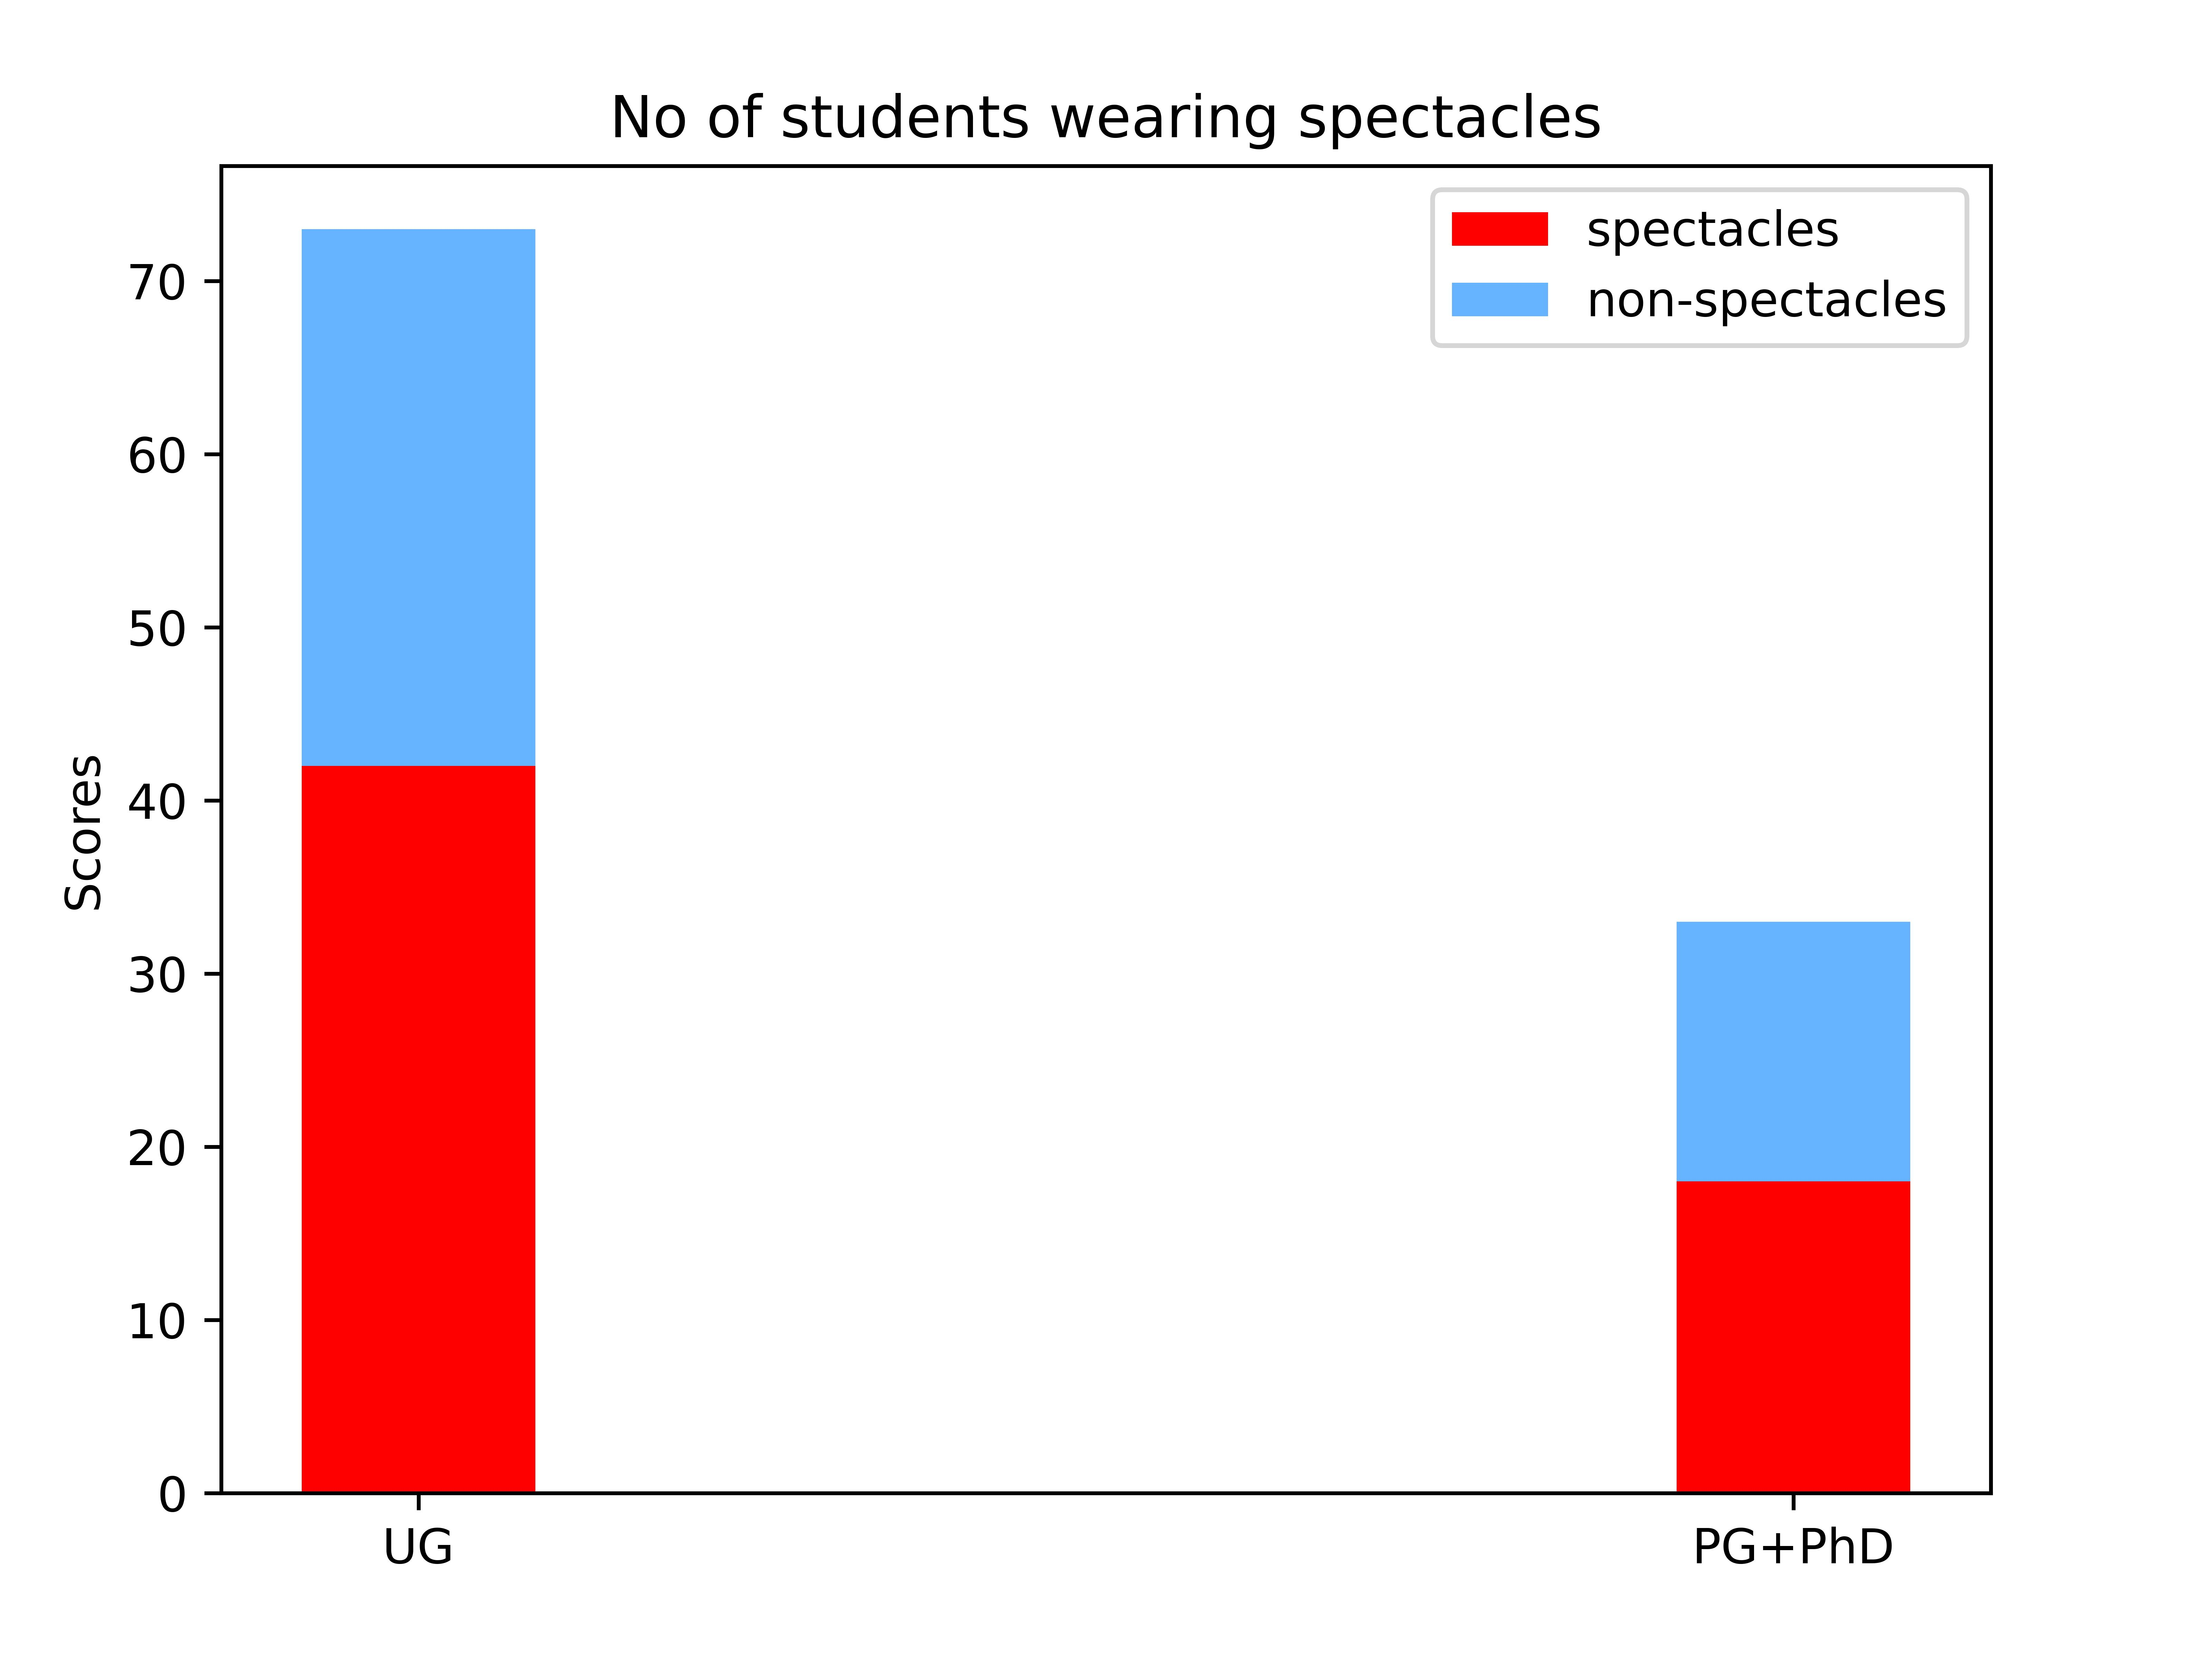
\includegraphics[scale=0.5]{no_of_students having_specs.jpg}
\end{figure}
\end{block}
\end{frame}

\begin{frame}
\begin{block}{Students in survey from different hostels}
\begin{figure}[hbtp]
\caption{Count of students from different hostel}
\centering
\includegraphics[height = 6cm, width=1.0\textwidth]{Number_of_students_vs_hostel.jpg}
\end{figure}
\end{block}
\end{frame}

\begin{frame}
\begin{block}{Students from different years}
\begin{figure}[hbtp]
\caption{Students from different years}
\centering
\includegraphics[width = 1.0\textwidth, height=6cm]{year_vs_Number_of_students.png}
\end{figure}
\end{block}
\end{frame}

\begin{frame}
\begin{block}{Study-time in one go v/s no. of students}
\begin{figure}[hbtp]
\caption{study-time in one go[categorial groups] v/s no. of students in that category}
\centering
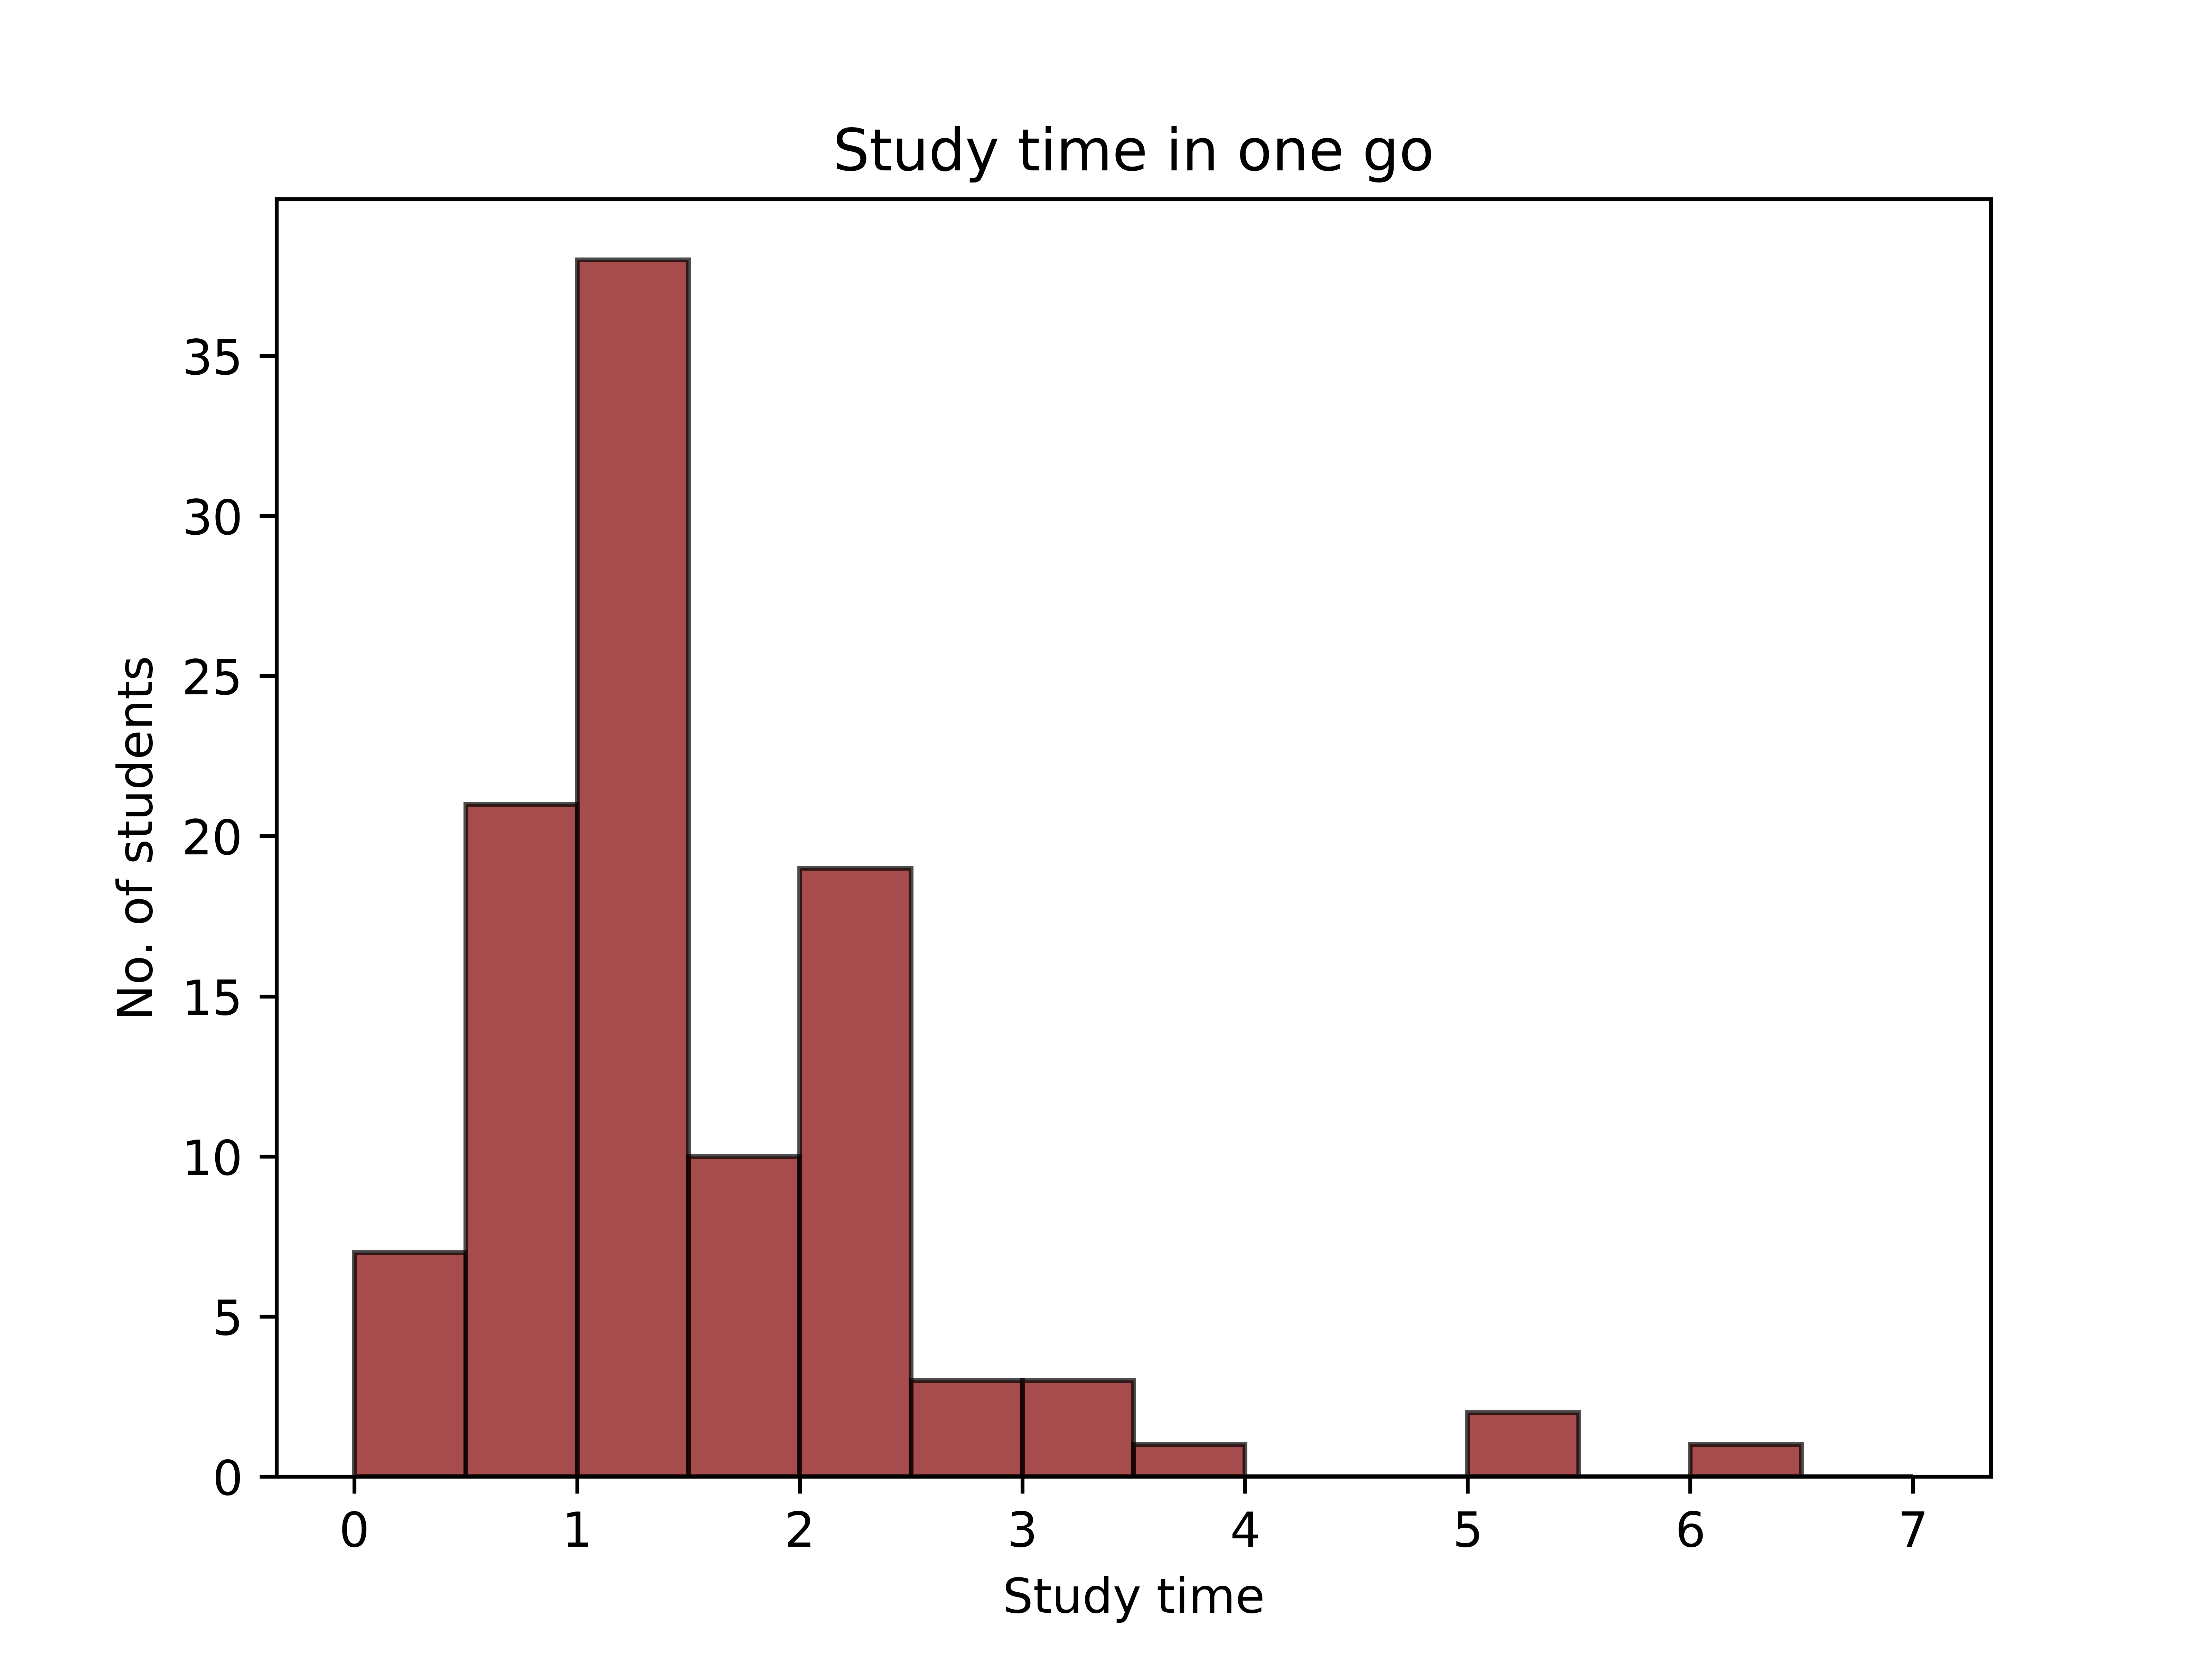
\includegraphics[scale=0.50]{Study time in one go.png}
\end{figure}
\end{block}
\end{frame}

\begin{frame}
\begin{block}{Productive screen time (percentage) distribution}
\begin{figure}[hbtp]
\caption{Productive screen-time [categorial groups size = 10] v/s number of students in group}
\centering
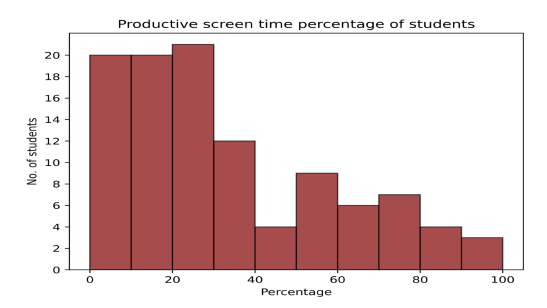
\includegraphics[width = 0.9\textwidth, height=6cm]{productive_screen_time.png}
\end{figure}
\end{block}
\end{frame}

\begin{frame}
\begin{block}{Happiness index v/s students}
\begin{figure}[hbtp]
\caption{Happiness index[1 to 5] v/s students}
\centering
\includegraphics[width=1.0\textwidth, height = 6cm]{Happiness_vs_number_of_students.png}
\end{figure}
\end{block}
\end{frame}


\begin{frame}
\begin{block}{Box-plot for the screen-time of students}
\begin{figure}[hbtp]
\caption{box-plot of screen-time of students}
\centering
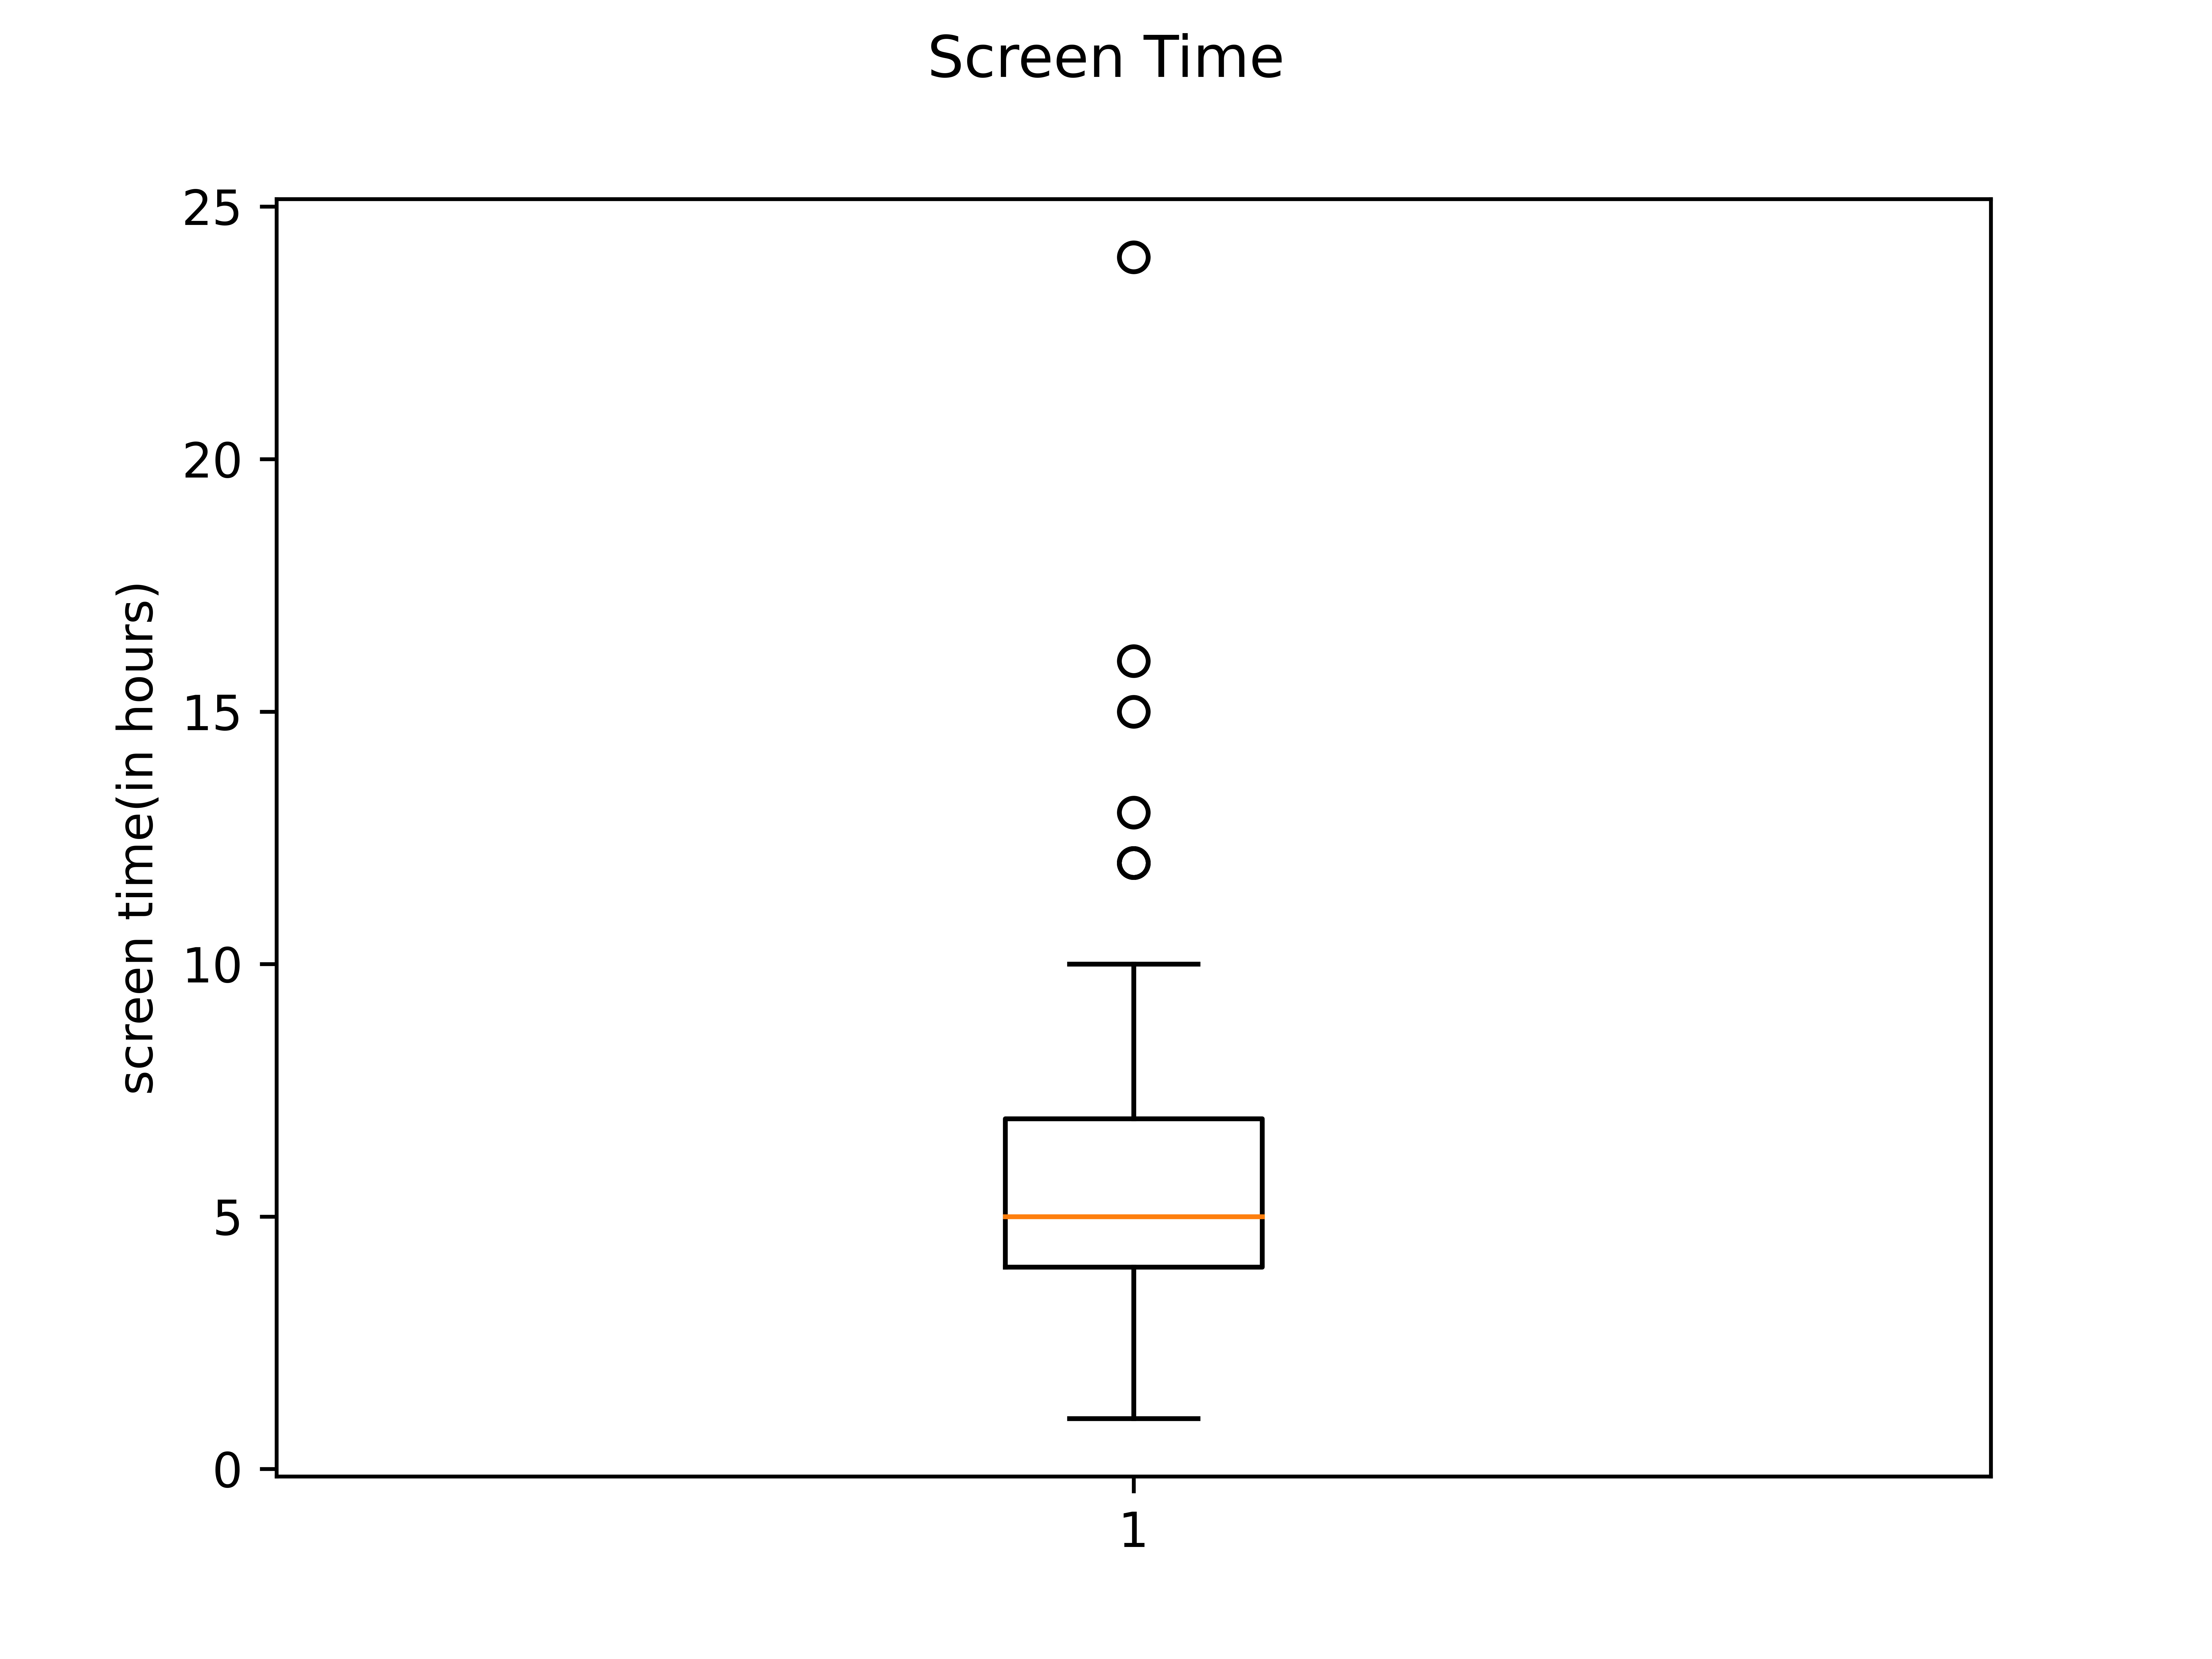
\includegraphics[scale=0.55]{boxplot.png}
\end{figure}
\end{block}
\end{frame}

\begin{frame}
\begin{block}{Distribution of screen-time among the students}
\begin{figure}[hbtp]
\caption{Distribution of students v/s screen time}
\centering
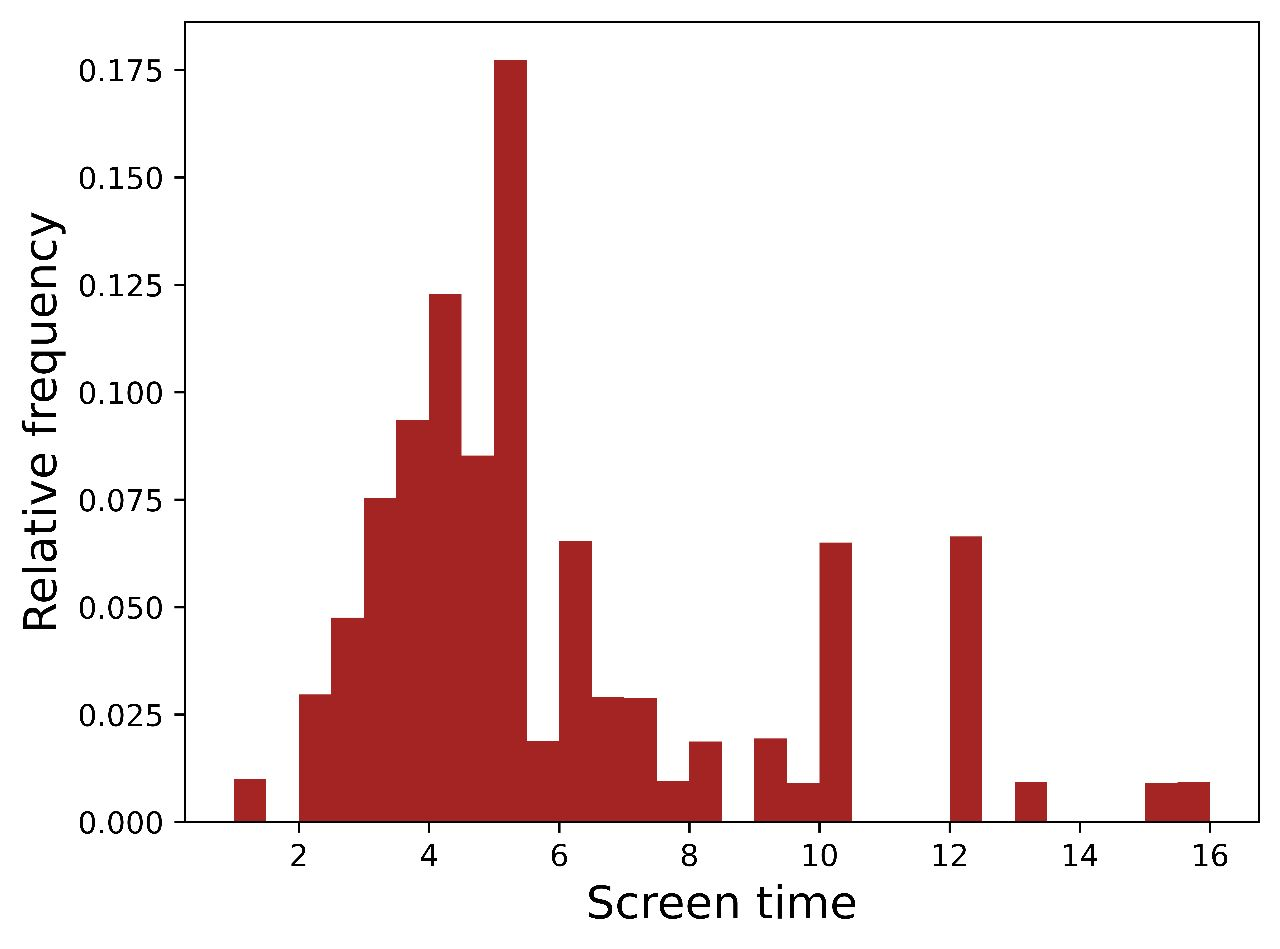
\includegraphics[scale=0.20]{population.png}
\end{figure}
\end{block}
\end{frame}

\begin{frame}
\begin{block}{Inference}
\begin{enumerate}
\item 70.75\% people have screen-time between 2 to 6 hours. 
\item While 28.3\% people have screen-time more than 6 hours.
\item And a very few percentage of people, i.e., 0.94\% have screen-time less than 2 hours.
\end{enumerate}
\end{block}
\end{frame}

\begin{frame}{Confidence Interval}
\begin{block}{Formula}
Let $\bar{x}$ = Sample Mean of target variable  \\
Let $S^2$ = Sample Variance of target variable \\
let  n= size of sample  
\\The Confidence interval is given by:
      \begin{align}
      [\bar{x} - E,\bar{x} + E]
 \end{align}
Where, E(Margin of Error) is given by,
 \begin{align}
      E =t_{{\alpha}, n-1}(\cfrac{S}{\sqrt{n}})
 \end{align}
 Width of the Confidence Interval is given by, $W = 2E$
\end{block}
\end{frame}

\begin{frame}{Confidence Interval}
\begin{block}{Case 1 : People with specs}
Based on the sample selected, we have the following information-
\begin{align}
    \bar{x} &= 6.68 \text{ hours}\\ 
    S &= 3.99\\
    n &= 60
\end{align}
Where, E(Margin of Error) is given by,
\\For 95\% Confidence Interval
\begin{center}
    $\alpha = 0.05$
\end{center}
\begin{align}
    E =t_{{\alpha}, n-1}(\cfrac{S}{\sqrt{n}})=t_{{0.05}, 59}(\cfrac{3.99}{\sqrt{60}})=2.0010(\cfrac{3.99}{\sqrt{60}})=1.030
\end{align}

 Width of the Confidence Interval is given by, $W = 2E= 2.06$.
\end{block}
\end{frame}
\begin{frame}{Confidence Interval}
\begin{block}{Case 1 : People with specs}
95\% Confidence Interval
 \begin{align}
      (\bar{x} - E,\bar{x} + E) = (5.65,7.71)
 \end{align}
 Similarly, The 99\% confidence interval is given by: 
 \begin{align}(5.31,8.05)\end{align} \\The width of the interval is given by: 2.74
 \newline
\\Therefore we can say with 95\% confidence that people who wear specs have average screen time between 5.65 and 7.71 hours
 \newline
\\And with 99\% confidence that people who wear specs have average screen time between 5.31 and 8.05 hours
\end{block}
\end{frame}

\begin{frame}{Confidence Interval}
\begin{block}{Case 2 : People without specs}
Based on the sample selected, we have the following information-
\begin{align}
    \bar{x} &=  5.03 \text{ hours}\\ 
    S &= 2.54\\
    n &= 46
\end{align}
Where, E(Margin of Error) is given by,
\\For 95\% Confidence Interval
\begin{center} 
    $\alpha = 0.05$
\end{center}
\begin{align}
    E =t_{{\alpha}, n-1}(\cfrac{S}{\sqrt{n}})=t_{{0.05}, 45}(\cfrac{3.99}{\sqrt{60}})=2.0141(\cfrac{5.03}{\sqrt{46}})=0.75
\end{align}

 Width of the Confidence Interval is given by, $W = 2E= 1.51$.
\end{block}
\end{frame}
\begin{frame}{Confidence Interval}
\begin{block}{Case 2 : People without specs}
95\% Confidence Interval
 \begin{align}
      (\bar{x} - E,\bar{x} + E) = (4.27,5.78)
 \end{align}
 Similarly, The 99\% confidence interval is given by: 
 \begin{align}(4.02,6.03)\end{align} \\The width of the interval is given by: 2.01
 \newline
\\Therefore we can say with 95\% confidence that people who wear specs have average screen time between 4.27 and 5.78 hours
 \newline
\\And with 99\% confidence that people who wear specs have average screen time between 4.02 and 6.03 hours
\end{block}
\end{frame}


\begin{frame}{Confidence Interval}
\begin{block}{Confidence Interval of Variance:}
Let $\bar{x}$ = Sample Mean of target variable  \\
Let $S^2$ = Sample Variance of target variable \\
let  n= size of same  
\\If $X_{1}, X_{2}, ..., X_{n}$ are normally distributed and $a = \chi^2_{(1-\frac{\alpha}{2},n-1)}$ and $b = \chi^2_{(\frac{\alpha}{2},n-1)}$, then a $(1-\alpha)100\%$ confidence interval for the population variance $\sigma^2$ is given by:

\begin{align}
\left(\frac{(n-1)S^2}{b},\frac{(n-1)S^2}{a}\right)
\end{align}
\end{block}
\end{frame}

\begin{frame}{Confidence Interval}
\begin{block}{Case 3 : Confidence interval of Variance of Screen-time}
Based on the sample selected, we have the following information-
\begin{align}
    S &= 3.52\\
    n &= 106\\
    a &= \chi^2_{(1-\frac{\alpha}{2},n-1)}= \chi^2_{(1-\frac{0.05}{2},105)}  = 78.54\\
    b &= \chi^2_{(\frac{\alpha}{2},n-1)} = \chi^2_{(\frac{0.05}{2},105)} = 135.25 
\end{align}
\end{block}
\end{frame}
\begin{frame}{Confidence Interval}
\begin{block}{Case 3 : Confidence interval of Variance of Screen-time}
95\% Confidence Interval
 \begin{gather}
      (\frac{(n-1)S^2}{b},\frac{(n-1)S^2}{a})\\
      (\frac{(105)12.3904}{135.25},\frac{(105)12.3904}{78.54})\\
      (9.62,16.57)
 \end{gather}
\\Therefore we can say with 95\% confidence that variance of average screen time of students lies between 9.62 and 16.57.
\end{block}
\end{frame}

\begin{frame}{Confidence Interval}
\begin{block}{Confidence Interval of Proportion:}
Let $\hat{p}$ = Sample Proportion
\\\text{Let  n= size of sample size}
\\
        \\\text{For large Random samples, a }\text{100\%} \text{CI for the Population proportion p is given by :}
        
      \begin{align}
      \left(\hat{p}-z_{\frac{\alpha}{2}}\sqrt{\frac{\hat{p}(1-\hat{p})}{n}},\hat{p}+z_{\frac{\alpha}{2}}\sqrt{\frac{\hat{p}(1-\hat{p})}{n}}\right)
 \end{align}

\end{block}
\end{frame}

\begin{frame}{Confidence Interval}
\begin{block}{Case 4 :  Confidence interval for Proportion of students who use phone between 4 to 6 hours :}
Based on the sample selected, we have the following information-
\begin{align}
    \hat{p} &= 0.47\\
    n &= 106
\end{align}
\end{block}
\end{frame}
\begin{frame}{Confidence Interval}
\begin{block}{Case 4 :  Confidence interval for Proportion of students who use phone for 4 to 6 hours :}
95\% Confidence Interval :
 \begin{gather}
      \left(\hat{p}-z_{\frac{\alpha}{2}}\sqrt{\frac{\hat{p}(1-\hat{p})}{n}},\hat{p}+z_{\frac{\alpha}{2}}\sqrt{\frac{\hat{p}(1-\hat{p})}{n}}\right)
      \\\left(0.47-z_{0.025}\sqrt{\frac{0.47(0.53)}{106}},0.47+z_{0.025}\sqrt{\frac{0.47(0.53)}{106}}\right)
      \\(0.3767,0.5667)
 \end{gather}
 \newline
\\Therefore we can say with 95\% confidence that the proportion of people using phone for 4 to 6 hours is between 0.3767 and 0.5667.
\end{block}
\end{frame}









\begin{frame}{Hypothesis Testings}
\begin{block}{Case 1: Comparing the screen time of people who attend all classes and those who don't attend all the classes}
\textbf{Null hypothesis} : People who attend all the classes have higher screen time compared to people who don't.\\
  $ H_0 : \mu_1 - \mu_2 \geq 0$ and $H_a : \mu_1 - \mu_2 < 0$
\par
\begin{center}
    $\bar{x_1} = 5.33$ hours \quad $\bar{x_2} = 6.67$ hours \\
    $S^2_1 = 2.90$ \quad
    $S^2_2 = 3.95$ \\
    $n_1 = 56$ \quad
    $n_2 = 50$
\end{center}
Since $\cfrac{S_1^2}{S_2^2} = 0.734 > 0.25$, we can assume the population variances are nearly equal.\\
The degrees of freedom, $df = n_1 + n_2 -2 = 104$, and the pooled variance will be:
\end{block}
\end{frame}

\begin{frame}{Hypothesis Testings}
\begin{block}{Case 1: Continued}

 \begin{align}
     S_p^2 &= \cfrac{(n_1-1)S_1^2 + (n_2-1)S_2^2}{n_1+n_2-2} = 11.8
 \end{align}
The test statistic $t$ is then given by:
\begin{align}
      t &= \cfrac{\bar{x_1} - \bar{x_2} - 0}{s_p\sqrt{\cfrac{1}{n_1} + \cfrac{1}{n_2}}} = -1.995\\ \end{align}
 Using the rejection region approach, we reject $H_0$ if $t \leq -t_{0.05, 104}$, where $t_{0.05,104} =1.658$. 
 Because the observed value of $t=-1.995$ is less than $-1.658$, we have enough statistical evidence to reject the null hypothesis, and thus, we can say, those who regularly go to class have less screen time on average than those who don't go to classes regularly.
\end{block}
\end{frame}

\begin{frame}{Hypothesis Testings}
\begin{block}{Case 2: Comparing the screen time of people with specs and people with no specs}
\textbf{Null hypothesis} :people who wear specs have less screen time compared to people who don't wear specs.\\
  $ H_0 : \mu_1 - \mu_2 \geq 0$ and $H_a : \mu_1 - \mu_2 < 0$
\par
\begin{center}
    $\bar{x_1} = 5.027$ hours \quad $\bar{x_2} = 6.683$ hours \\
    $S^2_1 = 6.453$ \quad
    $S^2_2 = 15.934$ \\
    $n_1 = 60$ \quad
    $n_2 = 46$
\end{center}
Since $\cfrac{S_1^2}{S_2^2} = 0.40 > 0.25$, we can assume the population variances are nearly equal.
\end{block}
\end{frame}

\begin{frame}{Hypothesis Testings}
\begin{block}{Case 2: Continued}
The degrees of freedom, $df = n_1 + n_2 -2 = 104$, and the pooled variance will be:
 \begin{align}
     S_p^2 &= \cfrac{(n_1-1)S_1^2 + (n_2-1)S_2^2}{n_1+n_2-2} = 10.5556
 \end{align}
The test statistic $t$ is then given by:
\begin{align}
      t = -2.601
 \end{align}
Using the rejection region approach, we reject $H_0$ if $t \leq -t_{0.05, 104}$, where $t_{0.05,104} = -1.659$.\\ 
 Because the observed value of $t=-2.601$ is less than $-1.659$, we have enough statistical evidence to reject the null hypothesis, and thus, we can say, those with specs have more screen time on average than those with no specs
\end{block}
\end{frame}

\begin{frame}{Hypothesis Testings}
\begin{block}{Case 3: Comparing variance in screen time of UG and PG + PHD}
\textbf{Null hypothesis}: The Variance in screen-time of UG is higher than Variance in screen-time of PG + PHD.\\



 For Hypothesis Testing, we make the following statements -

\par
\begin{center}
    \\
   $H_{0}: \sigma_{1}^{2} \geq \sigma_{2}^{2}$  and  $H_{a}: \sigma_{1}^{2} < \sigma_{2}^{2}$ \\
  
   $s_{1}^{2}=7.388$ \quad   $s_{2}^{2}= 22.279$\\
          $n_1 = 73$ \quad
    $n_2 = 33$  
    
    $df_{2}=n_{2}-1$  $df_{1}=n_{1}-1$  \\
   
\end{center}
\end{block}
\end{frame}

\begin{frame}{Hypothesis Testings}
\begin{block}{Case 3: Continued}
\begin{center}
         Test statistic: $F=\frac{s_{1}^{2}}{s_{2}^{2}}$\\
     $F=0.331$\\\
     $F_{1-\alpha, df_{1}, df_{2}}$=0.623\\
     \end{center}
 Rejection region: For a level $\alpha$ with degrees of freedom $df_{1}=n_{1}-1$ and $df_{2}=n_{2}-1$, reject $H_{0}$ if $F \leq F_{1-\alpha, df_{1}, df_{2}}$.\\
0.331 \leq 0.623\\
So we are able to reject the null hypothesis. So we can say the variance in screen-time of PG+PHD is greater than variance in screen-time of UG.\\
\end{block}
\end{frame}

\begin{frame}{Hypothesis Testings}
\begin{block} {Case 4:  Comparing the screen time of people who are unhappy and those
who are happy}
    \textbf{Null hypothesis} : people who are higher
on happiness metric $(\geq 3)$ have higher screen time than those who are lower on 
happiness metric $(\leq 2)$).

$ H_0 : \mu_1 - \mu_2 \geq 0$ and $H_a : \mu_1 - \mu_2 < 0$. Now, 
\par
\begin{center}
    $\bar{x_1} = 5.457$ hours \quad $\bar{x_2} = 7.897$ hours \\
    $S^2_1 = 3.2928$ \quad
    $S^2_2 = 3.6139$ \\
    $n_1 = 84$ \quad
    $n_2 = 22$
\end{center}

Since $\cfrac{S_1^2}{S_2^2} = 0.911>0.25$, we can assume the population variances are nearly equal.

\end{block}
\end{frame}

\begin{frame}{Hypothesis Testings}
\begin{block} {Case 4: Continued}
The degrees of freedom, $df = n_1 + n_2 -2 = 104$, and the pooled variance will be:
 \begin{align}
     S_p^2 &= \cfrac{(n_1-1)S_1^2 + (n_2-1)S_2^2}{n_1+n_2-2} = 3.357
 \end{align}
The test statistic $t$ is then given by:
 \begin{align}
      t &= \cfrac{\bar{x_1} - \bar{x_2} - 0}{s_p\sqrt{\cfrac{1}{n_1} + \cfrac{1}{n_2}}} = -3.03
 \end{align}
 \par
Using the rejection region approach, we reject $H_0$ if $t \leq -t_{0.05, 116}$, where $t_{0.05,116} = 1.658$.
Because the observed value of $t=-3.03$ is lesser than $-1.658$, we have enough statistical evidence to reject the null hypothesis, and thus, we can say, those who are higher on the happiness metric $(\geq 3)$  have lower screen time compared to people at lower happiness $(\leq 2)$.

\end{block}
\end{frame}

\begin{frame}{Takeaways from the analysis}
\begin{block}{From Confidence Intervals}
 \begin{enumerate}
    \item{Screentime vs Spectacles}
    \newline Mom was right, high screen time does make your eyesight weak. This was later confirmed by the Hypothesis testing.
    \item{Variance of Screentime data}
    \newline This gives us an idea of how much the data deviates from the mean.
    \item{Proportion of People who have Screentime between 4-6 hours}
    \newline Tells us that a sizable amount of the people use phone 4-6 hours daily.
\end{enumerate}
\end{block}
\end{frame}

\begin{frame}{Takeaways from the analysis}
\begin{block}{From Hypothesis Testings}
 \begin{enumerate}
    \item{Screentime and attendance}
    \newline Students who are regular in class have lower screen time than irregular students.
    \item{Screentime and Spectacles}
    \newline Students with spectacles were found to have higher average screen time than others.
    \item{Variance of Screentime data}
    \newline This gives us an idea of how much the data deviates from the mean.
    \ The variance of screen-time of PG/PHD is higher than that of UG.
    \item{Happiness and screen-time}
    \newline Students higher on happiness metric have lower average screen time than students on lower happiness metric.
\end{enumerate}
\end{block}
\end{frame}

\title{THANK YOU}
\begin{frame}
    \maketitle
\end{frame}

\end{document}
